
%% bare_conf.tex
%% V1.4b
%% 2015/08/26
%% by Michael Shell
%% See:
%% http://www.michaelshell.org/
%% for current contact information.
%%
%% This is a skeleton file demonstrating the use of IEEEtran.cls
%% (requires IEEEtran.cls version 1.8b or later) with an IEEE
%% conference paper.
%%
%% Support sites:
%% http://www.michaelshell.org/tex/ieeetran/
%% http://www.ctan.org/pkg/ieeetran
%% and
%% http://www.ieee.org/

%%*************************************************************************
%% Legal Notice:
%% This code is offered as-is without any warranty either expressed or
%% implied; without even the implied warranty of MERCHANTABILITY or
%% FITNESS FOR A PARTICULAR PURPOSE! 
%% User assumes all risk.
%% In no event shall the IEEE or any contributor to this code be liable for
%% any damages or losses, including, but not limited to, incidental,
%% consequential, or any other damages, resulting from the use or misuse
%% of any information contained here.
%%
%% All comments are the opinions of their respective authors and are not
%% necessarily endorsed by the IEEE.
%%
%% This work is distributed under the LaTeX Project Public License (LPPL)
%% ( http://www.latex-project.org/ ) version 1.3, and may be freely used,
%% distributed and modified. A copy of the LPPL, version 1.3, is included
%% in the base LaTeX documentation of all distributions of LaTeX released
%% 2003/12/01 or later.
%% Retain all contribution notices and credits.
%% ** Modified files should be clearly indicated as such, including  **
%% ** renaming them and changing author support contact information. **
%%*************************************************************************


% *** Authors should verify (and, if needed, correct) their LaTeX system  ***
% *** with the testflow diagnostic prior to trusting their LaTeX platform ***
% *** with production work. The IEEE's font choices and paper sizes can   ***
% *** trigger bugs that do not appear when using other class files.       ***                          ***
% The testflow support page is at:
% http://www.michaelshell.org/tex/testflow/



\documentclass[conference,a4paper]{IEEEtran}

% Some Computer Society conferences also require the compsoc mode option,
% but others use the standard conference format.
%
% If IEEEtran.cls has not been installed into the LaTeX system files,
% manually specify the path to it like:
% \documentclass[conference]{../sty/IEEEtran}





% Some very useful LaTeX packages include:
% (uncomment the ones you want to load)
\usepackage{siunitx}
\usepackage{tabularx}   % Tabellen, die sich automatisch der Breite anpassen
\usepackage{tabulary}   % Tabellen, die sich automatisch der Breite anpassen
\usepackage{booktabs}   % Verbesserte Möglichkeiten für Tabellenlayout über horizontale Linien
\usepackage{calculator}
\usepackage{subcaption}
\usepackage{multirow}
\usepackage{textcomp}
\usepackage{orcidlink}
\usepackage{cleveref}
\usepackage{wrapfig}
\usepackage{pgf}
\usepackage{graphicx}
\usepackage{makecell}
\usepackage[backend=biber, style=ieee, url=false]{biblatex}
\usepackage{url}
\addbibresource{Master.bib}
\newcommand{\squeezeup}{\vspace{-2mm}}


% *** MISC UTILITY PACKAGES ***
%
%\usepackage{ifpdf}
% Heiko Oberdiek's ifpdf.sty is very useful if you need conditional
% compilation based on whether the output is pdf or dvi.
% usage:
% \ifpdf
%   % pdf code
% \else
%   % dvi code
% \fi
% The latest version of ifpdf.sty can be obtained from:
% http://www.ctan.org/pkg/ifpdf
% Also, note that IEEEtran.cls V1.7 and later provides a builtin
% \ifCLASSINFOpdf conditional that works the same way.
% When switching from latex to pdflatex and vice-versa, the compiler may
% have to be run twice to clear warning/error messages.






% *** CITATION PACKAGES ***
%
%\usepackage{cite}
% cite.sty was written by Donald Arseneau
% V1.6 and later of IEEEtran pre-defines the format of the cite.sty package
% \cite{} output to follow that of the IEEE. Loading the cite package will
% result in citation numbers being automatically sorted and properly
% "compressed/ranged". e.g., [1], [9], [2], [7], [5], [6] without using
% cite.sty will become [1], [2], [5]--[7], [9] using cite.sty. cite.sty's
% \cite will automatically add leading space, if needed. Use cite.sty's
% noadjust option (cite.sty V3.8 and later) if you want to turn this off
% such as if a citation ever needs to be enclosed in parenthesis.
% cite.sty is already installed on most LaTeX systems. Be sure and use
% version 5.0 (2009-03-20) and later if using hyperref.sty.
% The latest version can be obtained at:
% http://www.ctan.org/pkg/cite
% The documentation is contained in the cite.sty file itself.






% *** GRAPHICS RELATED PACKAGES ***
%
\ifCLASSINFOpdf
  % \usepackage[pdftex]{graphicx}
  % declare the path(s) where your graphic files are
  % \graphicspath{{../pdf/}{../jpeg/}}
  % and their extensions so you won't have to specify these with
  % every instance of \includegraphics
  % \DeclareGraphicsExtensions{.pdf,.jpeg,.png}
\else
  % or other class option (dvipsone, dvipdf, if not using dvips). graphicx
  % will default to the driver specified in the system graphics.cfg if no
  % driver is specified.
  % \usepackage[dvips]{graphicx}
  % declare the path(s) where your graphic files are
  % \graphicspath{{../eps/}}
  % and their extensions so you won't have to specify these with
  % every instance of \includegraphics
  % \DeclareGraphicsExtensions{.eps}
\fi
% graphicx was written by David Carlisle and Sebastian Rahtz. It is
% required if you want graphics, photos, etc. graphicx.sty is already
% installed on most LaTeX systems. The latest version and documentation
% can be obtained at: 
% http://www.ctan.org/pkg/graphicx
% Another good source of documentation is "Using Imported Graphics in
% LaTeX2e" by Keith Reckdahl which can be found at:
% http://www.ctan.org/pkg/epslatex
%
% latex, and pdflatex in dvi mode, support graphics in encapsulated
% postscript (.eps) format. pdflatex in pdf mode supports graphics
% in .pdf, .jpeg, .png and .mps (metapost) formats. Users should ensure
% that all non-photo figures use a vector format (.eps, .pdf, .mps) and
% not a bitmapped formats (.jpeg, .png). The IEEE frowns on bitmapped formats
% which can result in "jaggedy"/blurry rendering of lines and letters as
% well as large increases in file sizes.
%
% You can find documentation about the pdfTeX application at:
% http://www.tug.org/applications/pdftex





% *** MATH PACKAGES ***
%
%\usepackage{amsmath}
% A popular package from the American Mathematical Society that provides
% many useful and powerful commands for dealing with mathematics.
%
% Note that the amsmath package sets \interdisplaylinepenalty to 10000
% thus preventing page breaks from occurring within multiline equations. Use:
%\interdisplaylinepenalty=2500
% after loading amsmath to restore such page breaks as IEEEtran.cls normally
% does. amsmath.sty is already installed on most LaTeX systems. The latest
% version and documentation can be obtained at:
% http://www.ctan.org/pkg/amsmath





% *** SPECIALIZED LIST PACKAGES ***
%
%\usepackage{algorithmic}
% algorithmic.sty was written by Peter Williams and Rogerio Brito.
% This package provides an algorithmic environment fo describing algorithms.
% You can use the algorithmic environment in-text or within a figure
% environment to provide for a floating algorithm. Do NOT use the algorithm
% floating environment provided by algorithm.sty (by the same authors) or
% algorithm2e.sty (by Christophe Fiorio) as the IEEE does not use dedicated
% algorithm float types and packages that provide these will not provide
% correct IEEE style captions. The latest version and documentation of
% algorithmic.sty can be obtained at:
% http://www.ctan.org/pkg/algorithms
% Also of interest may be the (relatively newer and more customizable)
% algorithmicx.sty package by Szasz Janos:
% http://www.ctan.org/pkg/algorithmicx




% *** ALIGNMENT PACKAGES ***
%
%\usepackage{array}
% Frank Mittelbach's and David Carlisle's array.sty patches and improves
% the standard LaTeX2e array and tabular environments to provide better
% appearance and additional user controls. As the default LaTeX2e table
% generation code is lacking to the point of almost being broken with
% respect to the quality of the end results, all users are strongly
% advised to use an enhanced (at the very least that provided by array.sty)
% set of table tools. array.sty is already installed on most systems. The
% latest version and documentation can be obtained at:
% http://www.ctan.org/pkg/array


% IEEEtran contains the IEEEeqnarray family of commands that can be used to
% generate multiline equations as well as matrices, tables, etc., of high
% quality.




% *** SUBFIGURE PACKAGES ***
%\ifCLASSOPTIONcompsoc
%  \usepackage[caption=false,font=normalsize,labelfont=sf,textfont=sf]{subfig}
%\else
%  \usepackage[caption=false,font=footnotesize]{subfig}
%\fi
% subfig.sty, written by Steven Douglas Cochran, is the modern replacement
% for subfigure.sty, the latter of which is no longer maintained and is
% incompatible with some LaTeX packages including fixltx2e. However,
% subfig.sty requires and automatically loads Axel Sommerfeldt's caption.sty
% which will override IEEEtran.cls' handling of captions and this will result
% in non-IEEE style figure/table captions. To prevent this problem, be sure
% and invoke subfig.sty's "caption=false" package option (available since
% subfig.sty version 1.3, 2005/06/28) as this is will preserve IEEEtran.cls
% handling of captions.
% Note that the Computer Society format requires a larger sans serif font
% than the serif footnote size font used in traditional IEEE formatting
% and thus the need to invoke different subfig.sty package options depending
% on whether compsoc mode has been enabled.
%
% The latest version and documentation of subfig.sty can be obtained at:
% http://www.ctan.org/pkg/subfig




% *** FLOAT PACKAGES ***
%
%\usepackage{fixltx2e}
% fixltx2e, the successor to the earlier fix2col.sty, was written by
% Frank Mittelbach and David Carlisle. This package corrects a few problems
% in the LaTeX2e kernel, the most notable of which is that in current
% LaTeX2e releases, the ordering of single and double column floats is not
% guaranteed to be preserved. Thus, an unpatched LaTeX2e can allow a
% single column figure to be placed prior to an earlier double column
% figure.
% Be aware that LaTeX2e kernels dated 2015 and later have fixltx2e.sty's
% corrections already built into the system in which case a warning will
% be issued if an attempt is made to load fixltx2e.sty as it is no longer
% needed.
% The latest version and documentation can be found at:
% http://www.ctan.org/pkg/fixltx2e


%\usepackage{stfloats}
% stfloats.sty was written by Sigitas Tolusis. This package gives LaTeX2e
% the ability to do double column floats at the bottom of the page as well
% as the top. (e.g., "\begin{figure*}[!b]" is not normally possible in
% LaTeX2e). It also provides a command:
%\fnbelowfloat
% to enable the placement of footnotes below bottom floats (the standard
% LaTeX2e kernel puts them above bottom floats). This is an invasive package
% which rewrites many portions of the LaTeX2e float routines. It may not work
% with other packages that modify the LaTeX2e float routines. The latest
% version and documentation can be obtained at:
% http://www.ctan.org/pkg/stfloats
% Do not use the stfloats baselinefloat ability as the IEEE does not allow
% \baselineskip to stretch. Authors submitting work to the IEEE should note
% that the IEEE rarely uses double column equations and that authors should try
% to avoid such use. Do not be tempted to use the cuted.sty or midfloat.sty
% packages (also by Sigitas Tolusis) as the IEEE does not format its papers in
% such ways.
% Do not attempt to use stfloats with fixltx2e as they are incompatible.
% Instead, use Morten Hogholm'a dblfloatfix which combines the features
% of both fixltx2e and stfloats:
%
% \usepackage{dblfloatfix}
% The latest version can be found at:
% http://www.ctan.org/pkg/dblfloatfix




% *** PDF, URL AND HYPERLINK PACKAGES ***
%
%\usepackage{url}
% url.sty was written by Donald Arseneau. It provides better support for
% handling and breaking URLs. url.sty is already installed on most LaTeX
% systems. The latest version and documentation can be obtained at:
% http://www.ctan.org/pkg/url
% Basically, \url{my_url_here}.




% *** Do not adjust lengths that control margins, column widths, etc. ***
% *** Do not use packages that alter fonts (such as pslatex).         ***
% There should be no need to do such things with IEEEtran.cls V1.6 and later.
% (Unless specifically asked to do so by the journal or conference you plan
% to submit to, of course. )


% correct bad hyphenation here
\hyphenation{op-tical net-works semi-conduc-tor}


\begin{document}
%
% paper title
% Titles are generally capitalized except for words such as a, an, and, as,
% at, but, by, for, in, nor, of, on, or, the, to and up, which are usually
% not capitalized unless they are the first or last word of the title.
% Linebreaks \\ can be used within to get better formatting as desired.
% Do not put math or special symbols in the title.
\title{Comparison of optical and capacitive\\ Dew Point Detection using COTS Components}



% \author{\IEEEauthorblockN{Malte Nilges}
% \IEEEauthorblockA{Integrated Electronic Systems Lab\\
% \textit{Technische Universität Darmstadt}\\
% Darmstadt, Germany\\
% malte.nilges@stud.tu-darmstadt.de}
% \and
% \IEEEauthorblockN{David Riehl}
% \IEEEauthorblockA{Integrated Electronic Systems Lab\\
% \textit{Technische Universität Darmstadt}\\
% Darmstadt, Germany\\
% david.riehl@ies.tu-darmstadt.de}
% \and
% \IEEEauthorblockN{Klaus Hofmann}
% \IEEEauthorblockA{Integrated Electronic Systems Lab\\
% \textit{Technische Universität Darmstadt}\\
% Darmstadt, Germany\\
% klaus.hofmann@ies.tu-darmstadt.de}
% \and
% \IEEEauthorblockN{Ferdinand Keil}
% \IEEEauthorblockA{Integrated Electronic Systems Lab\\
% \textit{Technische Universität Darmstadt}\\
% Darmstadt, Germany\\
% ferdinand.keil@ies.tu-darmstadt.de}}

\author{
\IEEEauthorblockN{Malte Nilges \orcidlink{0000-0001-9704-8390}, David Riehl \orcidlink{0000-0003-0513-7447}, Klaus Hofmann \orcidlink{0000-0002-6675-0221} and Ferdinand Keil \orcidlink{0000-0002-8970-309X}}
\IEEEauthorblockA{\textit{Integrated Electronic Systems Lab, Technische Universität Darmstadt, Germany}
\\
Malte.Nilges@gmail.com, Ferdinand.Keil@ies.tu-darmstadt.de, Klaus.Hofmann@ies.tu-darmstadt.de}}


% conference papers do not typically use \thanks and this command
% is locked out in conference mode. If really needed, such as for
% the acknowledgment of grants, issue a \IEEEoverridecommandlockouts
% after \documentclass

% for over three affiliations, or if they all won't fit within the width
% of the page, use this alternative format:
% 
%\author{\IEEEauthorblockN{Michael Shell\IEEEauthorrefmark{1},
%Homer Simpson\IEEEauthorrefmark{2},
%James Kirk\IEEEauthorrefmark{3}, 
%Montgomery Scott\IEEEauthorrefmark{3} and
%Eldon Tyrell\IEEEauthorrefmark{4}}
%\IEEEauthorblockA{\IEEEauthorrefmark{1}School of Electrical and Computer Engineering\\
%Georgia Institute of Technology,
%Atlanta, Georgia 30332--0250\\ Email: see http://www.michaelshell.org/contact.html}
%\IEEEauthorblockA{\IEEEauthorrefmark{2}Twentieth Century Fox, Springfield, USA\\
%Email: homer@thesimpsons.com}
%\IEEEauthorblockA{\IEEEauthorrefmark{3}Starfleet Academy, San Francisco, California 96678-2391\\
%Telephone: (800) 555--1212, Fax: (888) 555--1212}
%\IEEEauthorblockA{\IEEEauthorrefmark{4}Tyrell Inc., 123 Replicant Street, Los Angeles, California 90210--4321}}




% use for special paper notices
%\IEEEspecialpapernotice{(Invited Paper)}




% make the title area
\maketitle

% As a general rule, do not put math, special symbols or citations
% in the abstract
\begin{abstract}
This works presents a dew point temperature sensor employing parallel capacitive and optical readout of a chilled electroless nickel immersion gold (ENIG) surface. The use of commercial off the shelf (COTS) components and simple mechanical construction leads to a reproducible and cost-effective sensor system, which is put to test using saturated salt solutions in order to give a comprehensible comparison of capacitive and optical sensing methods. A multitude of sensors was put to test, including four temperature sensor models, two proximity sensors and an interdigital electrodes (IDE) capacitor.
\end{abstract}

\begin{IEEEkeywords}
  humidity, dew point, temperature sensor, cots, capacitance measurement, deliquescence
  \end{IEEEkeywords}
% no keywords




% For peer review papers, you can put extra information on the cover
% page as needed:
% \ifCLASSOPTIONpeerreview
% \begin{center} \bfseries EDICS Category: 3-BBND \end{center}
% \fi
%
% For peerreview papers, this IEEEtran command inserts a page break and
% creates the second title. It will be ignored for other modes.
\IEEEpeerreviewmaketitle



\section{Introduction}
% no \IEEEPARstart
Dew point hygrometers are crucial for accurately measuring atmospheric moisture in various industrial and scientific applications, such as meteorology and semiconductor manufacturing. Compared to other measurement principles they can provide high temperature ranges of several hundred degrees celsius, accuracies in the millidegree range and adaptability to different gas mixtures \autocite{korotcenkovHandbookHumidityMeasurement2019}. Most research in these devices has been performed in optical methods, which detect the condensation on chilled mirrors through changes in light intensity caused by scattering or absorption \autocite{korotcenkovHandbookHumidityMeasurement2019,chenHumiditySensorsReview2005,srivastavaHumiditySensorOverview2012}. While recent works involve new and precise techniques for dew point detection, such as a quartz oscillator \autocite{nieNewTypeFast2016} or a photonic resonator \autocite{taoUltrahighaccuracyMiniatureDew2016}, these methods require manufacturing of custom sensors, leading to high cost in case of low volume production. This paper examines and compares the use of optical and capacitive measurement methods for enabling low-cost dew point hygrometers.

% Optical dew point hygrometers use a chilled mirror to detect the temperature at which condensation forms, providing high accuracy and real-time measurements. Capacitive hygrometers, on the other hand, measure changes in capacitance of a hygroscopic material as it absorbs moisture, offering robustness and low power consumption.


\section{Examination of Temperature Sensors}
The temperature readout is a critical component of the sensor system, requiring high accuracy and fast response times as an error of \qty{0.1}{\K} can yield a deviation in relative humidity (RH) of up to \qty{1}{\percent}. An early test evaluated multiple temperature sensors to identify suitable candidates for the platform. The test used a Fluke 5615 platinum resistance thermometer (PRT), a Fluke 7320 calibration bath for temperature control and a Keysight 3458A multimeter. For a measurement duration of \qty{60}{\s} for each target temperature, the temperature sensors were read every \qty{200}{\milli\s} using a microcontroller and the reference temperature was determined every \qty{2}{\s} using a 4-wire resistance measurement of the PRT and its ITS-90 calibration coefficients. Based on the last recalibration cycle of approximately 3 years, the accuracy of the multimeter can be assumed to be \qty{\pm 5}{\milli\K} for the respective resistance measurement range of \qty{100}{\kilo\ohm}, and that of the PRT to be \qty{\pm 19}{\milli\K}. Four different types of temperature sensors were put to test: AMS AS6221, Silicon Labs Si7051, Analog Devices ADT7422 and TI TMP117; of each type four devices on a single \qtyproduct{35 x 45}{\mm} printed circuit board (PCB). The test temperatures ranged from \qtyrange{-10}{60}{\celsius} in steps of \qty{10}{\celsius}.

\begin{figure}
  \centering
  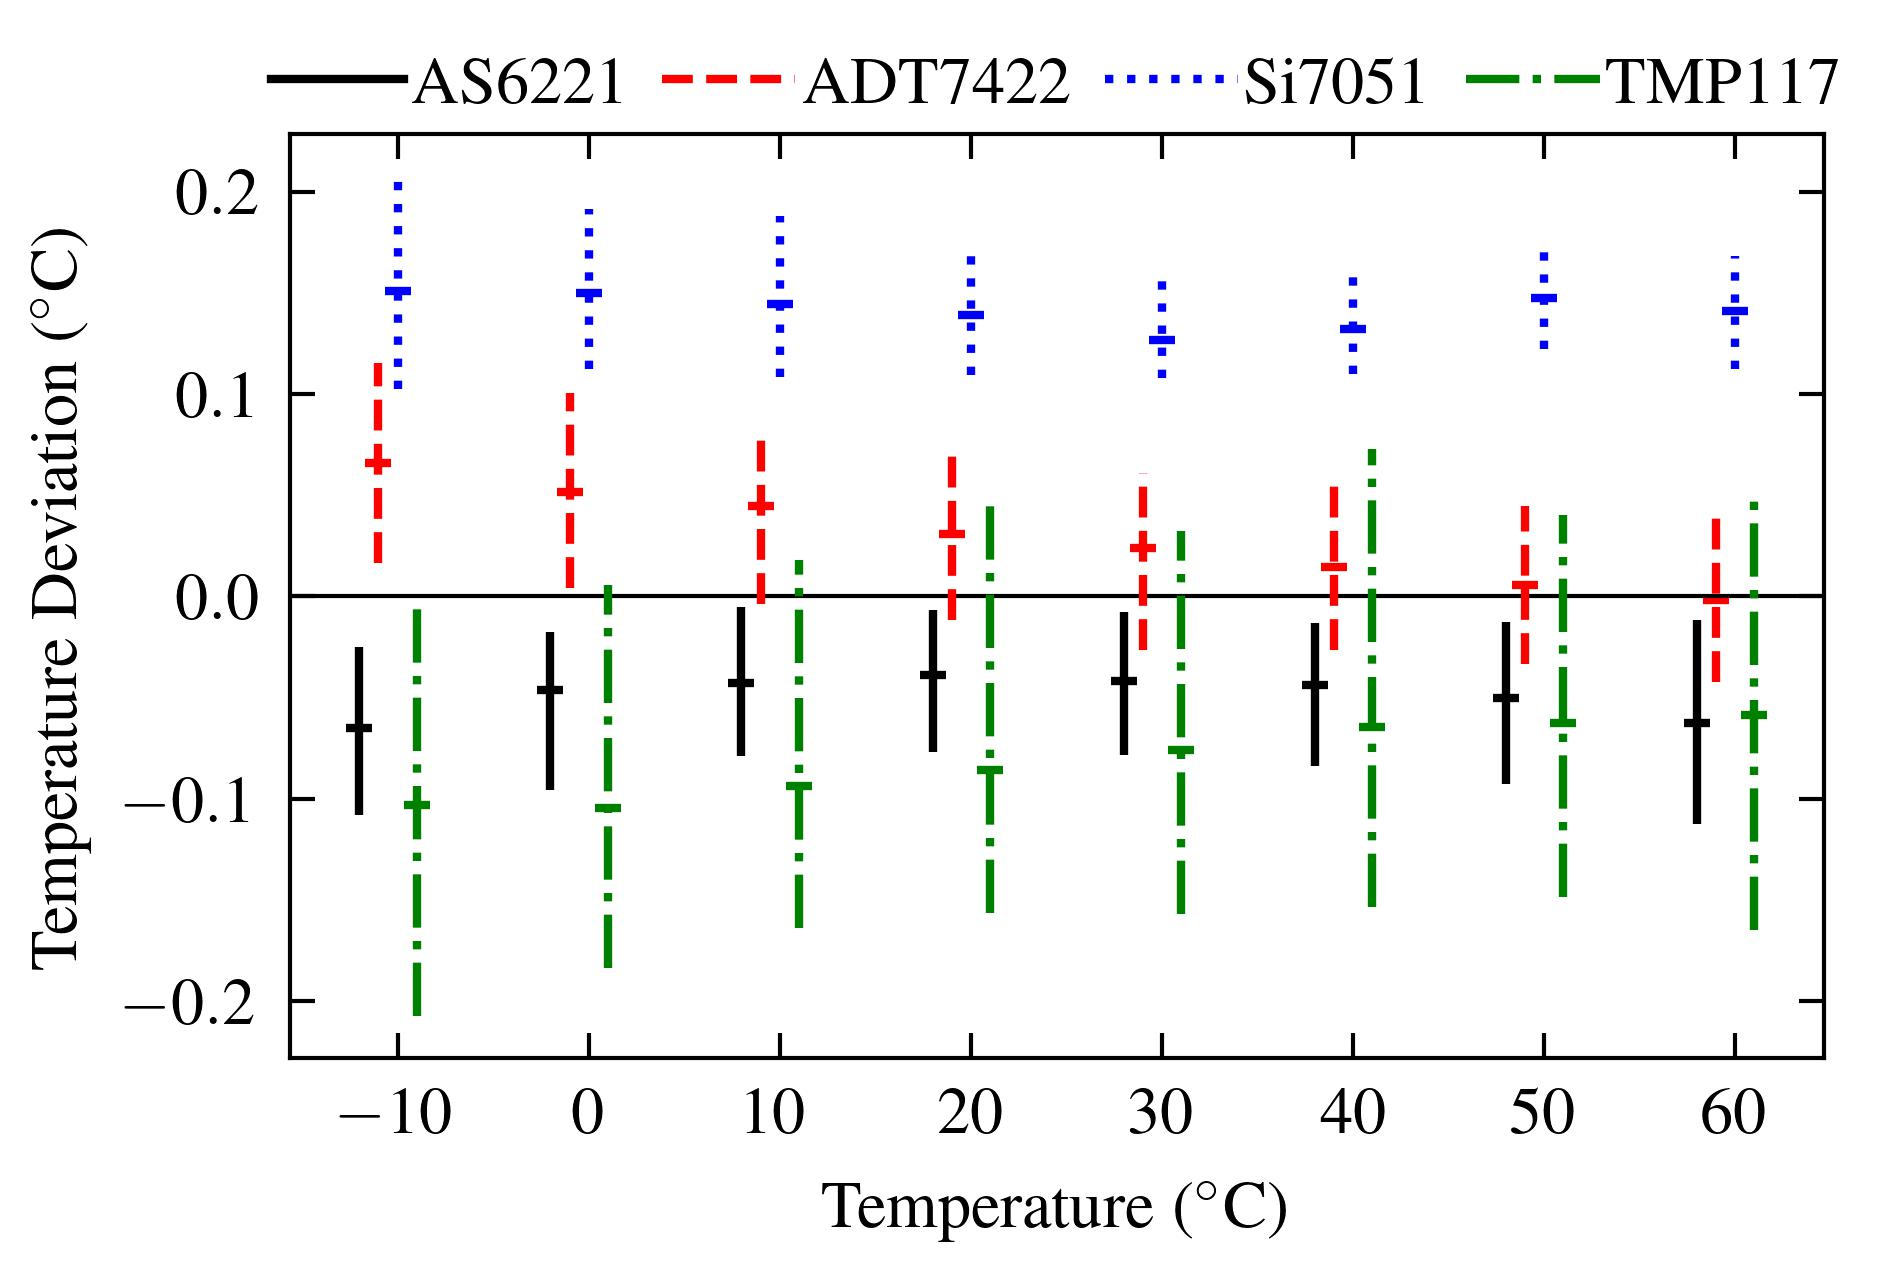
\includegraphics[width=\columnwidth]{graphs/tempsensors}
  \caption{Average, minimum and maximum temperature deviation of four devices of each temperature sensor model compared to the PRT.}
  \label{g:temp_dev}
  \squeezeup
\end{figure}


\Cref{g:temp_dev} shows the the average, minimum and maximum deviations in relation to the PRT reference, which itself deviated less than \qty{15}{\milli\K} during the complete measurement cycles.
The results show that only the ADT7422 and AS6221 sensors were able to consistently measure the temperature within their respective specifications of \qtylist{0.1;0.09}{\K}, with only few measurements exceeding the specification. The Si7051 devices had a consistent offset of around \qty[retain-explicit-plus]{+0.15}{\K}, leading to all measured devices being outside specification. The TMP117 devices were on average within specification, yet yielded most inconsistent temperature measurements, which may deviate around \qty{0.2}{\K} across timepoints and devices.

\section{Methods}
\subsection{Hardware}
The sensor platform is divided into two primary components: the base board and the mirror board. The base board integrates a cluster of proximity sensors, specifically the Vishay VCNL36825T, which utilizes a vertical cavity surface emitting laser with a narrow emission beam, and the Vishay VCNL4040, which employs an infrared light emitting diode (LED) with a broader emission beam.

The mirror board is designed as a flexible printed circuit (FPC) to minimize thermal resistance. It features an ENIG-coated copper surface which hosts an array of four Osram AS6221 temperature sensors. The surface is subdivided into one continuous part acting as a mirror surface for the proximity sensors and one interdigitated part acting as an IDE capacitor. A trace heater on the backside of the surface and a thermoelectric cooler mounted on top  provide uniform and rapid temperature adjustments. For the capacitor readout, a relaxation oscillator using a single TI SN74LVC1G14 inverting Schmitt trigger is employed, which charges and discharges the capacitor. Its switching frequency depends on the capacitance, giving a direct measure of dew.

\subsection{Software}
The control software was written for the STM32 microcontroller platform, involving the set-up of thresholds for dew point presence based on initial sensor readings and thereafter the execution of multiple cooling and reheating cycles. The first cycle determines a dew point temperature window based on the initial thresholds using a fast cool down in order to avoid lenghty and inefficient cooling. Subsequent cycles work within this window and decrease the cool down speed in order to achieve higher resolution in temperature readout. Within every cycle, cooling and heating of the copper surface is regulated by a proportional-integral-derivative (PID) controller at a frequency of \qty{5}{\Hz} using the average temperature reading of the four sensors. The temperature, frequency and proximity readings are transferred to a host computer.

For the following data analysis, the system employs the use of smoothing splines as a regression technique \autocite{ScipyInterpolateSplrep,dierckxAlgorithmSmoothingDifferentiation1975}. The splines use a minimal number of piecewise connected polynomials (B-splines) of $k$th degree to fit the resulting curve to the measurement data, adhering to an error constraint that was determined empirically for the measurement data. This allows for a reduction of high-frequency noise while offering a low amount of smoothing and delay in case of step changes in measurement data as compared to finite impulse response (FIR) filters using fixed window functions.

\subsection{Testing Environment}
In order to provide accurate measurements, a setup with salt solutions inside a properly sealed container was chosen to achieve a fixed-point humidity control. Four saturated salt solutions were used in a ventilated system for lowering the saturation vapour pressure as displayed in \Cref{t:equi}. The values for the vapour pressures have been extensively researched and provide reliable assumptions about the reference humidity in the test setup \autocite{greenspanHumidityFixedPoints1977}. Temperatures have been settled to an accuracy of \qty{\pm 0.1}{\K} and the ventilation was performed for at least three hours in order to achieve constant humidity.

% \begin{wraptable}{l}{1\textwidth}
\begin{table}
\caption{Equilibrium Relative Humidities \autocite{greenspanHumidityFixedPoints1977} and Measurement Errors of the Control Substances}
\label{t:equi}
\centering
\begin{tabular*}{\columnwidth}{@{\extracolsep{\fill}}r|ll|ccc}
    % \toprule
    \toprule
Substance                        & T (\unit{\celsius}) & RH ($\Delta$) (\unit{\percent}) & \multicolumn{3}{c}{Measured $\Delta$RH (\unit{\percent})}  \\
 & & & IDE & OPT1 & OPT2 \\
\midrule
\multirow{3}{*}{MgCl\textsubscript{2}}           & 10 *          & 33.47 (\textpm 0.24) &   -0.94 &   +0.06 &   +0.42 \\
& 25 *          & 32.78 (\textpm 0.16) &   +0.61 &   -0.57 &   +0.36 \\
& 40 *          & 31.60 (\textpm 0.13) &   -0.66 &   -0.87 &   -0.23 \\
\midrule
\multirow{3}{*}{\makecell{Mg(NO\textsubscript{3})\textsubscript{2}\\ * 6H\textsubscript{2}O}} & 10 *          & 57.36 (\textpm 0.33) &   +0.07 &   +0.11 &   +0.11 \\
& 25          & 52.89 (\textpm 0.22) &   +1.37 &   -1.68 &   +0.33 \\
& 40          & 48.42 (\textpm 0.37) &   +3.29 &   -1.46 &   +8.68 \\
\midrule
\multirow{3}{*}{NaCl}            & 10          & 75.67 (\textpm 0.22) &    -1.10 &   +1.04 &   +3.62 \\
& 25          & 75.29 (\textpm 0.12) &    +1.10 &   -3.02 &   +1.38 \\
& 40          & 74.68 (\textpm 0.13) &    +4.44 &   -1.48 &   -1.48 \\
\midrule
\multirow{3}{*}{K\textsubscript{2}SO\textsubscript{4}}           & 10          & 98.18 (\textpm 0.76) &    +4.18 &   +1.21 &   +1.08 \\
                                 & 25          & 97.59 (\textpm 0.53) &    -0.75 &   -4.00 &   -1.27 \\
                                 & 40          & 96.71 (\textpm 0.38) &    -2.97 &   -5.16 &   +0.34 \\
\midrule
\multicolumn{6}{c}{\makecell{OPT1: VNCL4040, OPT2: VCNL36825T, * change in setup}}
% \bottomrule
\end{tabular*}
\end{table}
% \end{wraptable}

\section{Results and Discussion}
\subsection{Dew Sensor Characterization}
The capacitive sensor is measured to have a capacitance of \qty{180}{\pico\F} at ambient temperature and humidity. It is charged and discharged through \qty{1}{\mega\ohm} resistors, the sampling frequency for the inverter circuitry is \qty{170}{\mega\Hz} and its thresholds \qtylist{1.05; 1.55}{\V}. This results in a period of $T_{RC} = \qty{115.34}{\us}$ or a frequency of \qty{8.67}{\kilo\Hz} using following equation \autocite{texasinstrumentsRelaxationOscillatorCircuit2018}:
\begin{equation}
    \label{e:cap_period}
    T = RC \cdot \ln\left[ \frac{(V_{DD}-V_{th,n})V_{th,p}}{(V_{DD}-V_{th,p})V_{th,n}}\right].
\end{equation}
With a sampling period of $T_{s} = \frac{1}{\qty{170}{\mega\Hz}} = \qty{5.88}{\ns}$, this results in a sensitivity of \qty{51}{ppm}, which is severely limited however by noise introduced into the measurement system such as fluctuations in supply and threshold voltage, fluctuations in sampling frequency, electromagnetic interference, temperature and mechanical forces. For noise estimation, the capacitive sensor was placed in a quasi-static environment according to external sensors ($\Delta T$ = \qty[retain-explicit-plus]{20}{\milli\K}, $\Delta RH$ = \qty[retain-explicit-plus]{0.3}{\percent}) for a duration of \qty{30}{\s}, resulting in a signal-to-noise ratio (SNR) of \qty{81.2}{\dB}.
%noise levels of less than \qty{-100}{\dB} at frequencies higher than \qty{0.15}{\Hz}, indicating stable short-term frequency measurements.

The optical sensors are specified to detect objects within a range of \qtyrange{0}{200}{\mm}, yet their output code at a given distance is different as to their different emitting power and angle. Both sensors yield 16 bit output codes which correlate to the amount of dew collected on the reflective surface. In the same test setup for noise estimation, the sensors yield optical readings with SNRs of \qty{70.3}{\dB} and \qty{71.3}{\dB} respectively.

\subsection{Initial Measurements}
The first test consisted of reading initial sensor measurements for the respective temperatures and humidities. The capacitive measurement is highly influenced by the humidity, as can be seen in \cref{g:cap_initial}. Lower relative humidities result in less capacitance and thus an increased switching frequency of the relaxation oscillator, whereas the temperature has no clear influence on the measurements for a fixed relative humidity. 
The optical measurements do not exhibit significant dependence on relative or absolute humidity.

\begin{figure}
  \centering
  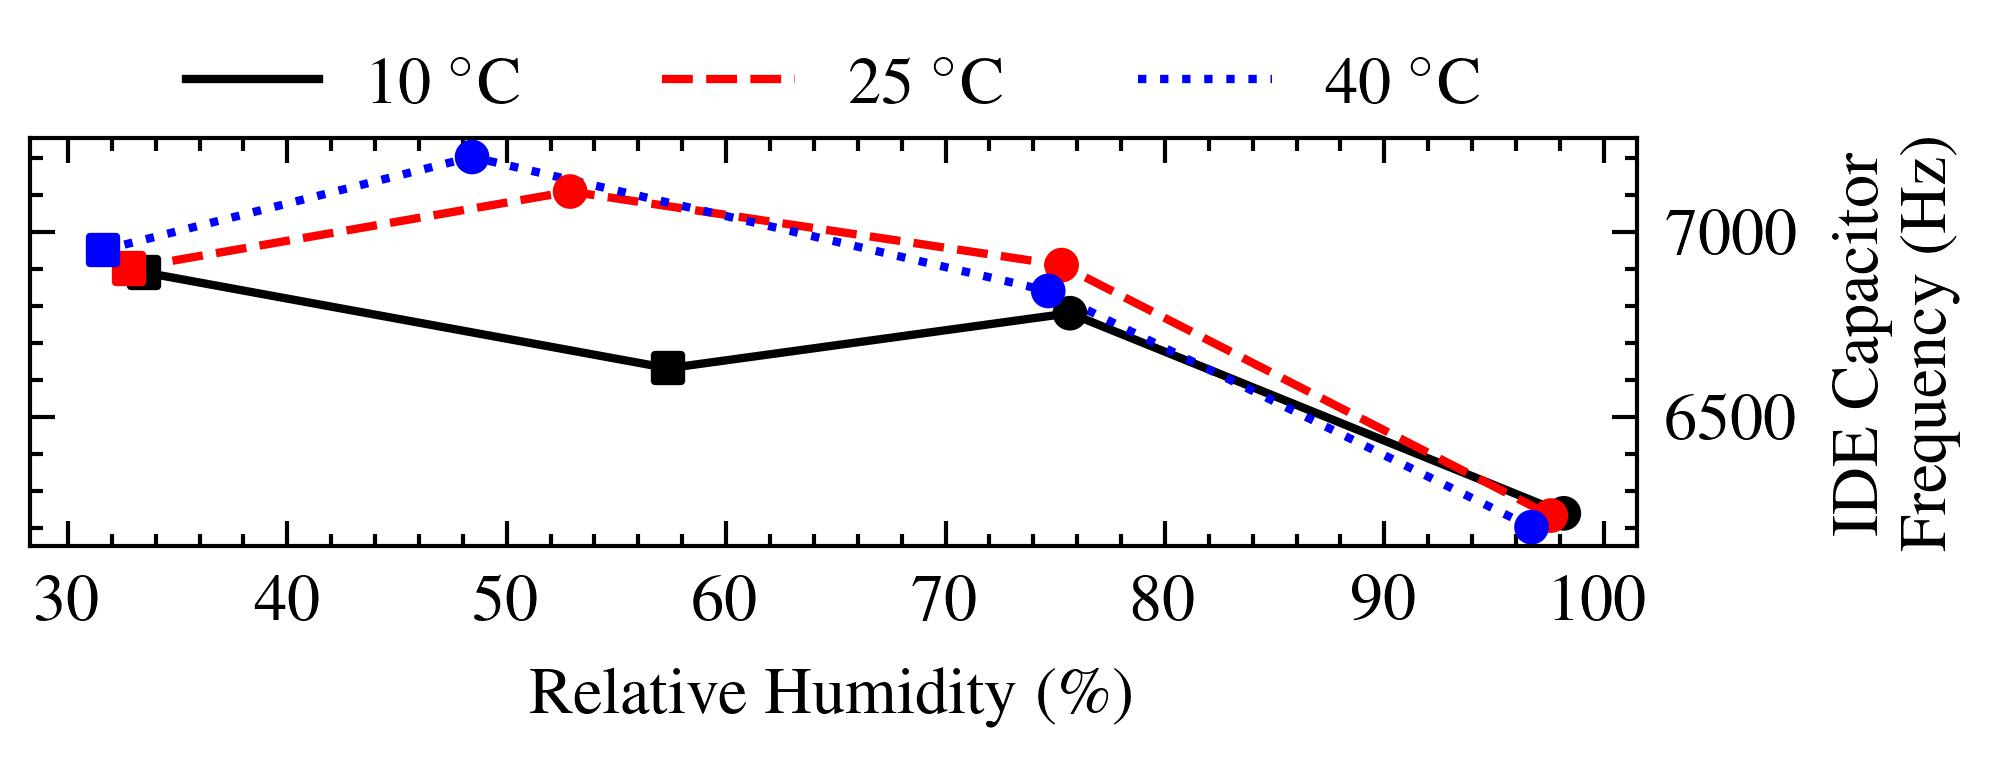
\includegraphics[width=\columnwidth]{graphs/cap_initial}
  \caption{Initial frequencies for the different measurements. Rectangular markers show the results after test setup changes.}
  \label{g:cap_initial}
\end{figure}

\subsection{Dew Point Detection}

\Cref{g:cap_t25rh50} shows the dew point measurement of the IDE capacitor and VCNL4040 in the test configuration of $T$ = \qty{25.0}{\celsius} and $RH$ = \qty{52.89}{\percent}. The measurement diagram of VCNL36825T is not shown due to space constraints, but resembles that of the VCNL4040. 

\begin{figure}
  \centering
  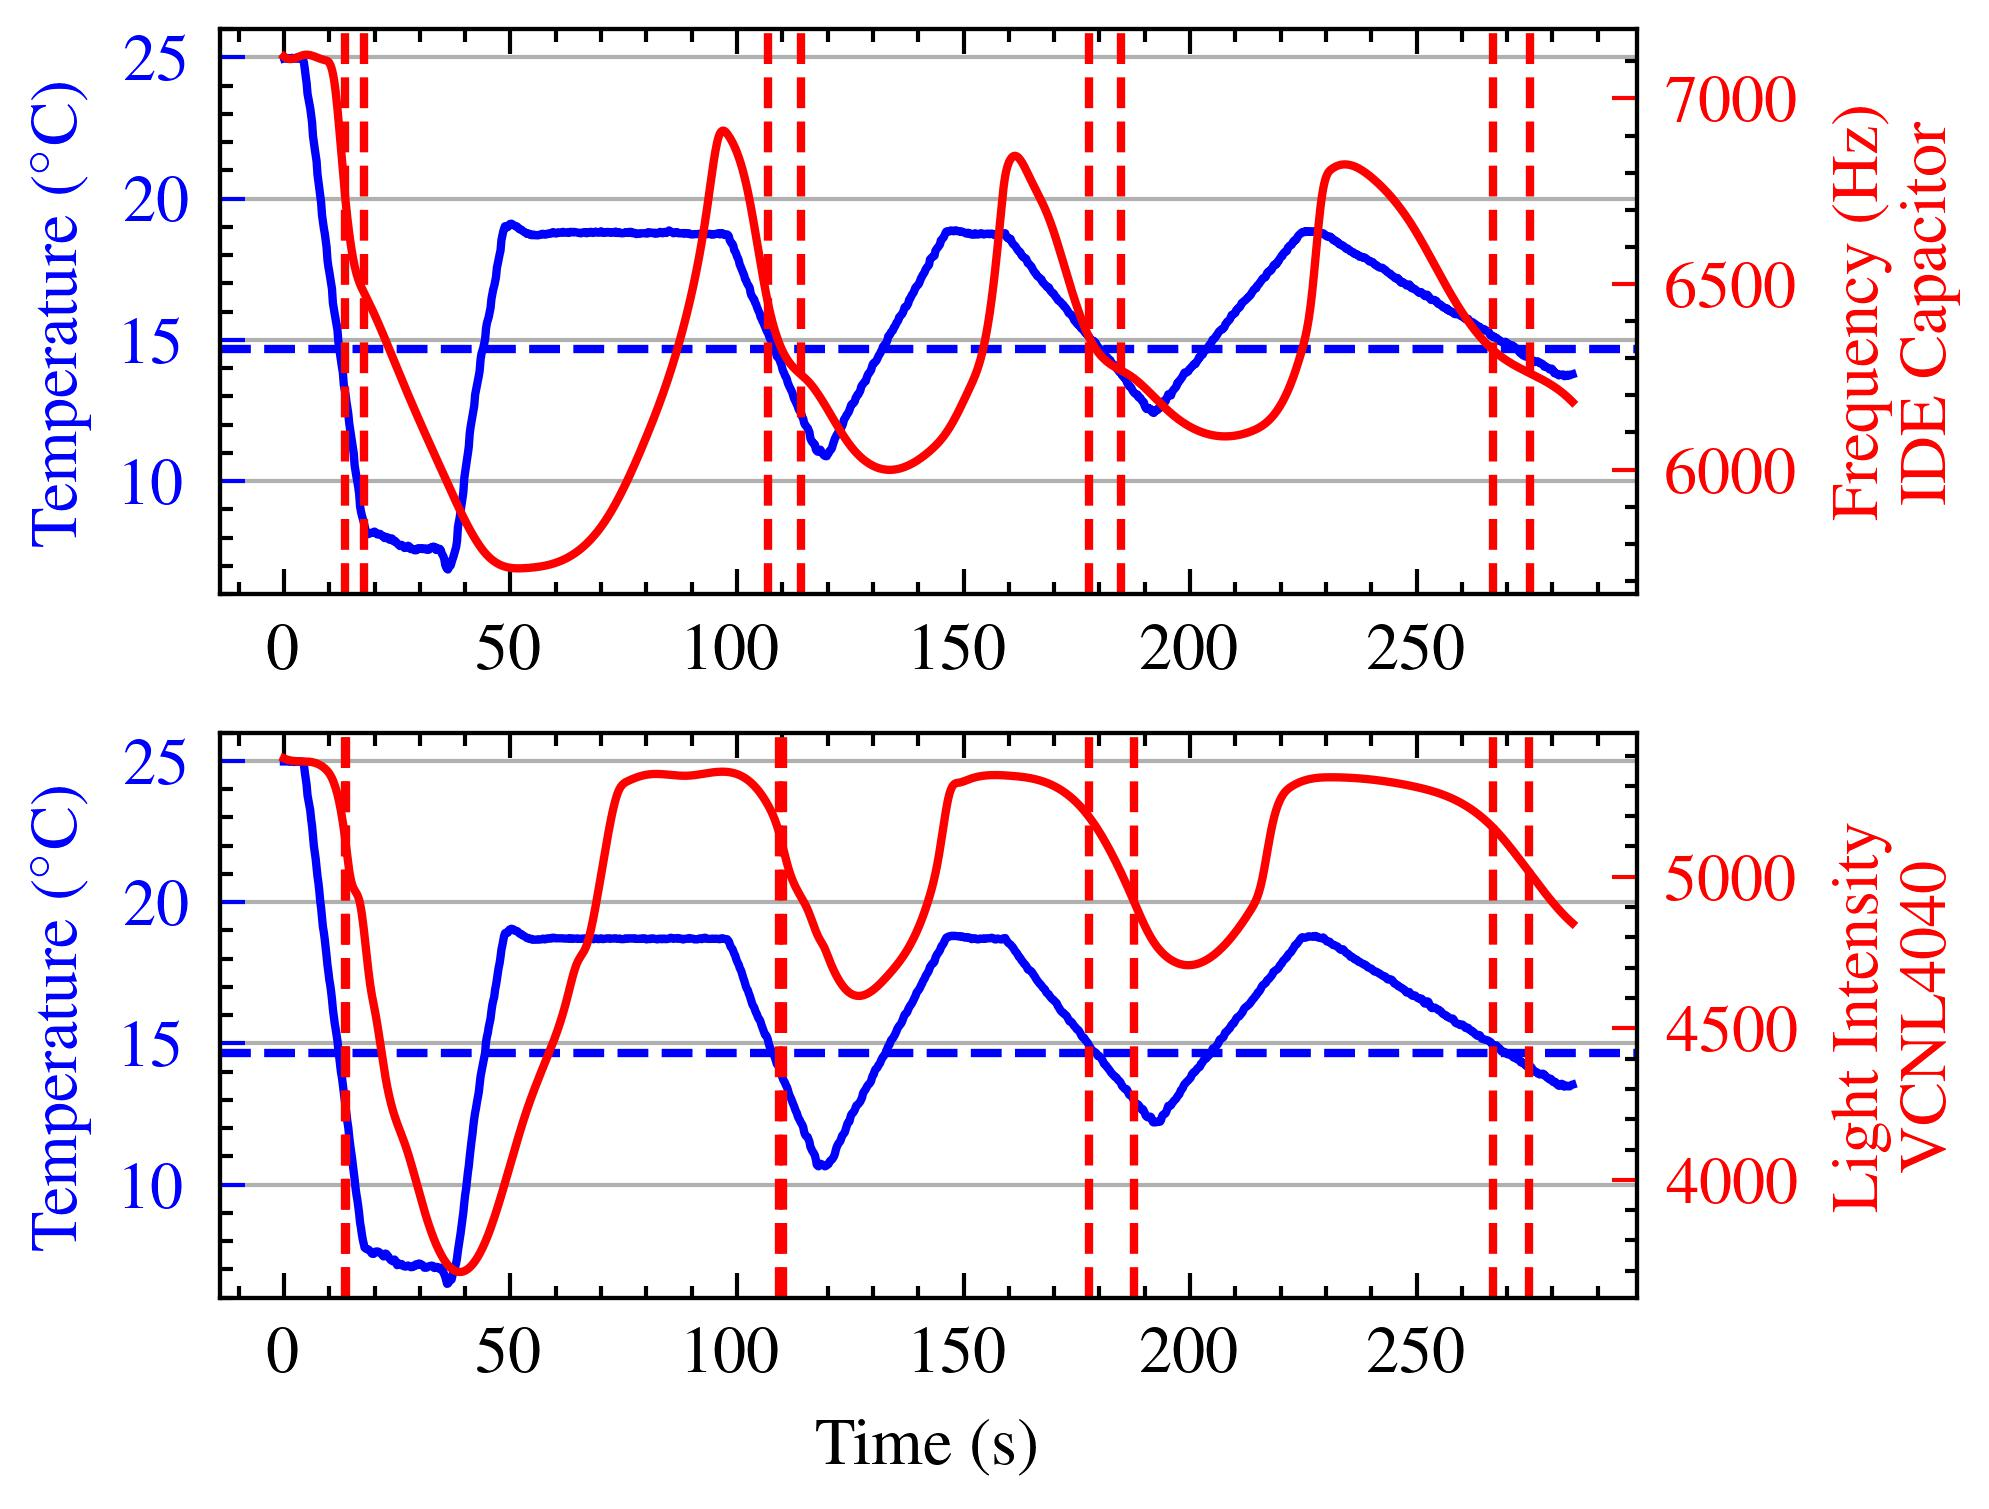
\includegraphics[width=\columnwidth]{graphs/cap_t25rh50}
  \caption{Measurement of the dew point temperature for $T$ = \qty{25.0}{\celsius}, $RH$ = \qty{52.89}{\percent}. The horizontal dashed lines indicate the actual dew point temperature, the vertical dashed lines indicate the determined dew point temperature range in each cooldown cycle (\qtylist[per-mode=fraction]{-1.3;-0.4; -0.2; -0.1}{\K\per\s}).}
  \label{g:cap_t25rh50}
  \squeezeup
\end{figure}

The first cooldown cycle is used for fast working dew point range detection, limiting the following cycles to only a few degrees celsius. The curves of the capacitive and optical sensors differ significantly throughout the measurement and hence require different analysis methods in order to determine the dew point temperature. The capacitive element is very sensitive even to smallest changes in temperature. As suggested by the results of the initial measurements, this may be caused by induced local changes of relative humidity. The dew point is marked by a small step in the frequency slope, hence it is determined to be within the timestamps of the maximum of the second derivative and the maximum of the first derivative. The frequency around the dew point differs significantly depending on the ambient temperature and humidity conditions.

Contrastingly, the output signal of the proximity sensors is much more stable until close to the dew point. As expected, right around the timepoint of condensation, there is a significant change in light intensity due to refraction and absorption caused by the water molecules. The dew point is found to be always within the minimum of the second derivative and the minimum of the first derivative.

\begin{figure}
  \centering
  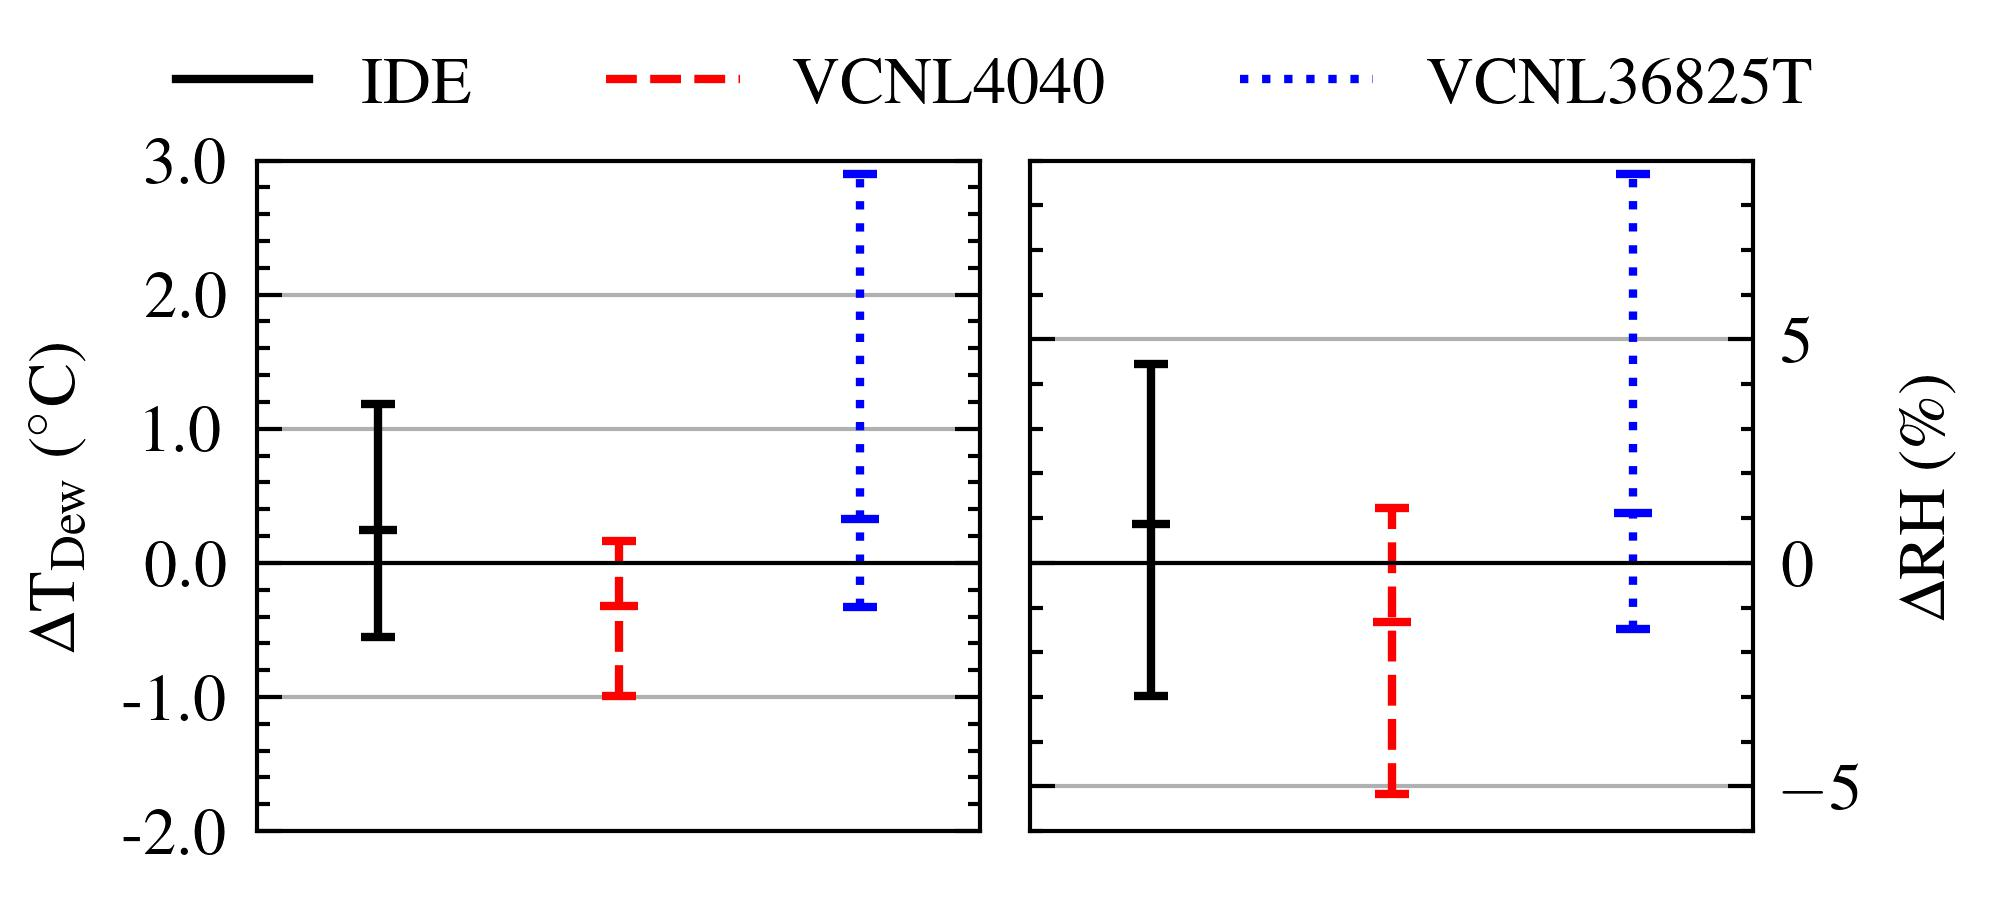
\includegraphics[width=\columnwidth]{graphs/sensorall_dew}
  \caption{Average, minimum and maximum measured dew point temperature and relative humidity deviation for each sensor.}
  \label{g:sensorall_dew}
  \squeezeup
\end{figure}

Due to the limited amount of test data, no interpolation techniques have been employed for improving the accuracy of the determined dew point temperature. Instead, the on average closest limiting temperature values of the last cycles have been chosen, that is for the capacitive sensor the start and for the optical sensors the end of the determined range. The resulting relative humidity errors for each sensor and measurement are shown in \cref{t:equi}. \Cref{g:sensorall_dew} shows the error range and the mean error over all measurements for each sensor. The error range of the measured dew point temperature is found to be around \qtylist{1.2;1.8}{\celsius} for the VCNL4040 and IDE capacitor respectively. This value is one order of magnitude higher than the accuracy of the used temperature sensor, indicating the dew point detection to be the limiting factor. A further decrease of cooldown speed for a higher resolution is unlikely to yield substantially higher accuracy, as the improvement compared to the previous cooldown cycle is already insignificant. Taking the large error range of around \qty{3.5}{\celsius} of the VCNL36825T into consideration, it is suggested that error detection schemes based on the found temperature range and a data-driven interpolation of the dew point within said range may need to be employed. Repeated measurements with real-time dew point analysis have the potential to ensure a sufficiently precise result.


\section{Conclusion}
The sensor platform employs the optical and capacitive dew point sensing in parallel and yields a comprehensive comparison of the underlying differences in readout. In the realized setup, there is no clear winner between the two principles, as both require careful interpretation of the acquired data to determine the exact timepoints of condensation. Using simple data analysis methods, the dew point could be determined with a deviation of less than \qty{1}{\celsius}. For higher accuracies, the use of more sophisticated data analysis methods and a real-time error estimation is suggested.

% trigger a \newpage just before the given reference
% number - used to balance the columns on the last page
% adjust value as needed - may need to be readjusted if
% the document is modified later
%\IEEEtriggeratref{8}
% The "triggered" command can be changed if desired:
%\IEEEtriggercmd{\enlargethispage{-5in}}

% references section

% can use a bibliography generated by BibTeX as a .bbl file
% BibTeX documentation can be easily obtained at:
% http://mirror.ctan.org/biblio/bibtex/contrib/doc/
% The IEEEtran BibTeX style support page is at:
% http://www.michaelshell.org/tex/ieeetran/bibtex/
%\bibliographystyle{IEEEtran}
% argument is your BibTeX string definitions and bibliography database(s)
%\bibliography{IEEEabrv,../bib/paper}
%
% <OR> manually copy in the resultant .bbl file
% set second argument of \begin to the number of references
% (used to reserve space for the reference number labels box)


% \urlstyle{rm}
% \setcounter{biburllcpenalty}{9000000}
% \setcounter{biburlucpenalty}{10000000}
% \emergencystretch 1.5em

\def\UrlBreaks{\do\/\do-}
\printbibliography




% that's all folks
\end{document}


